\chapter{Simulations} 


\section{r128} 

\subsection{drdx\_3} 

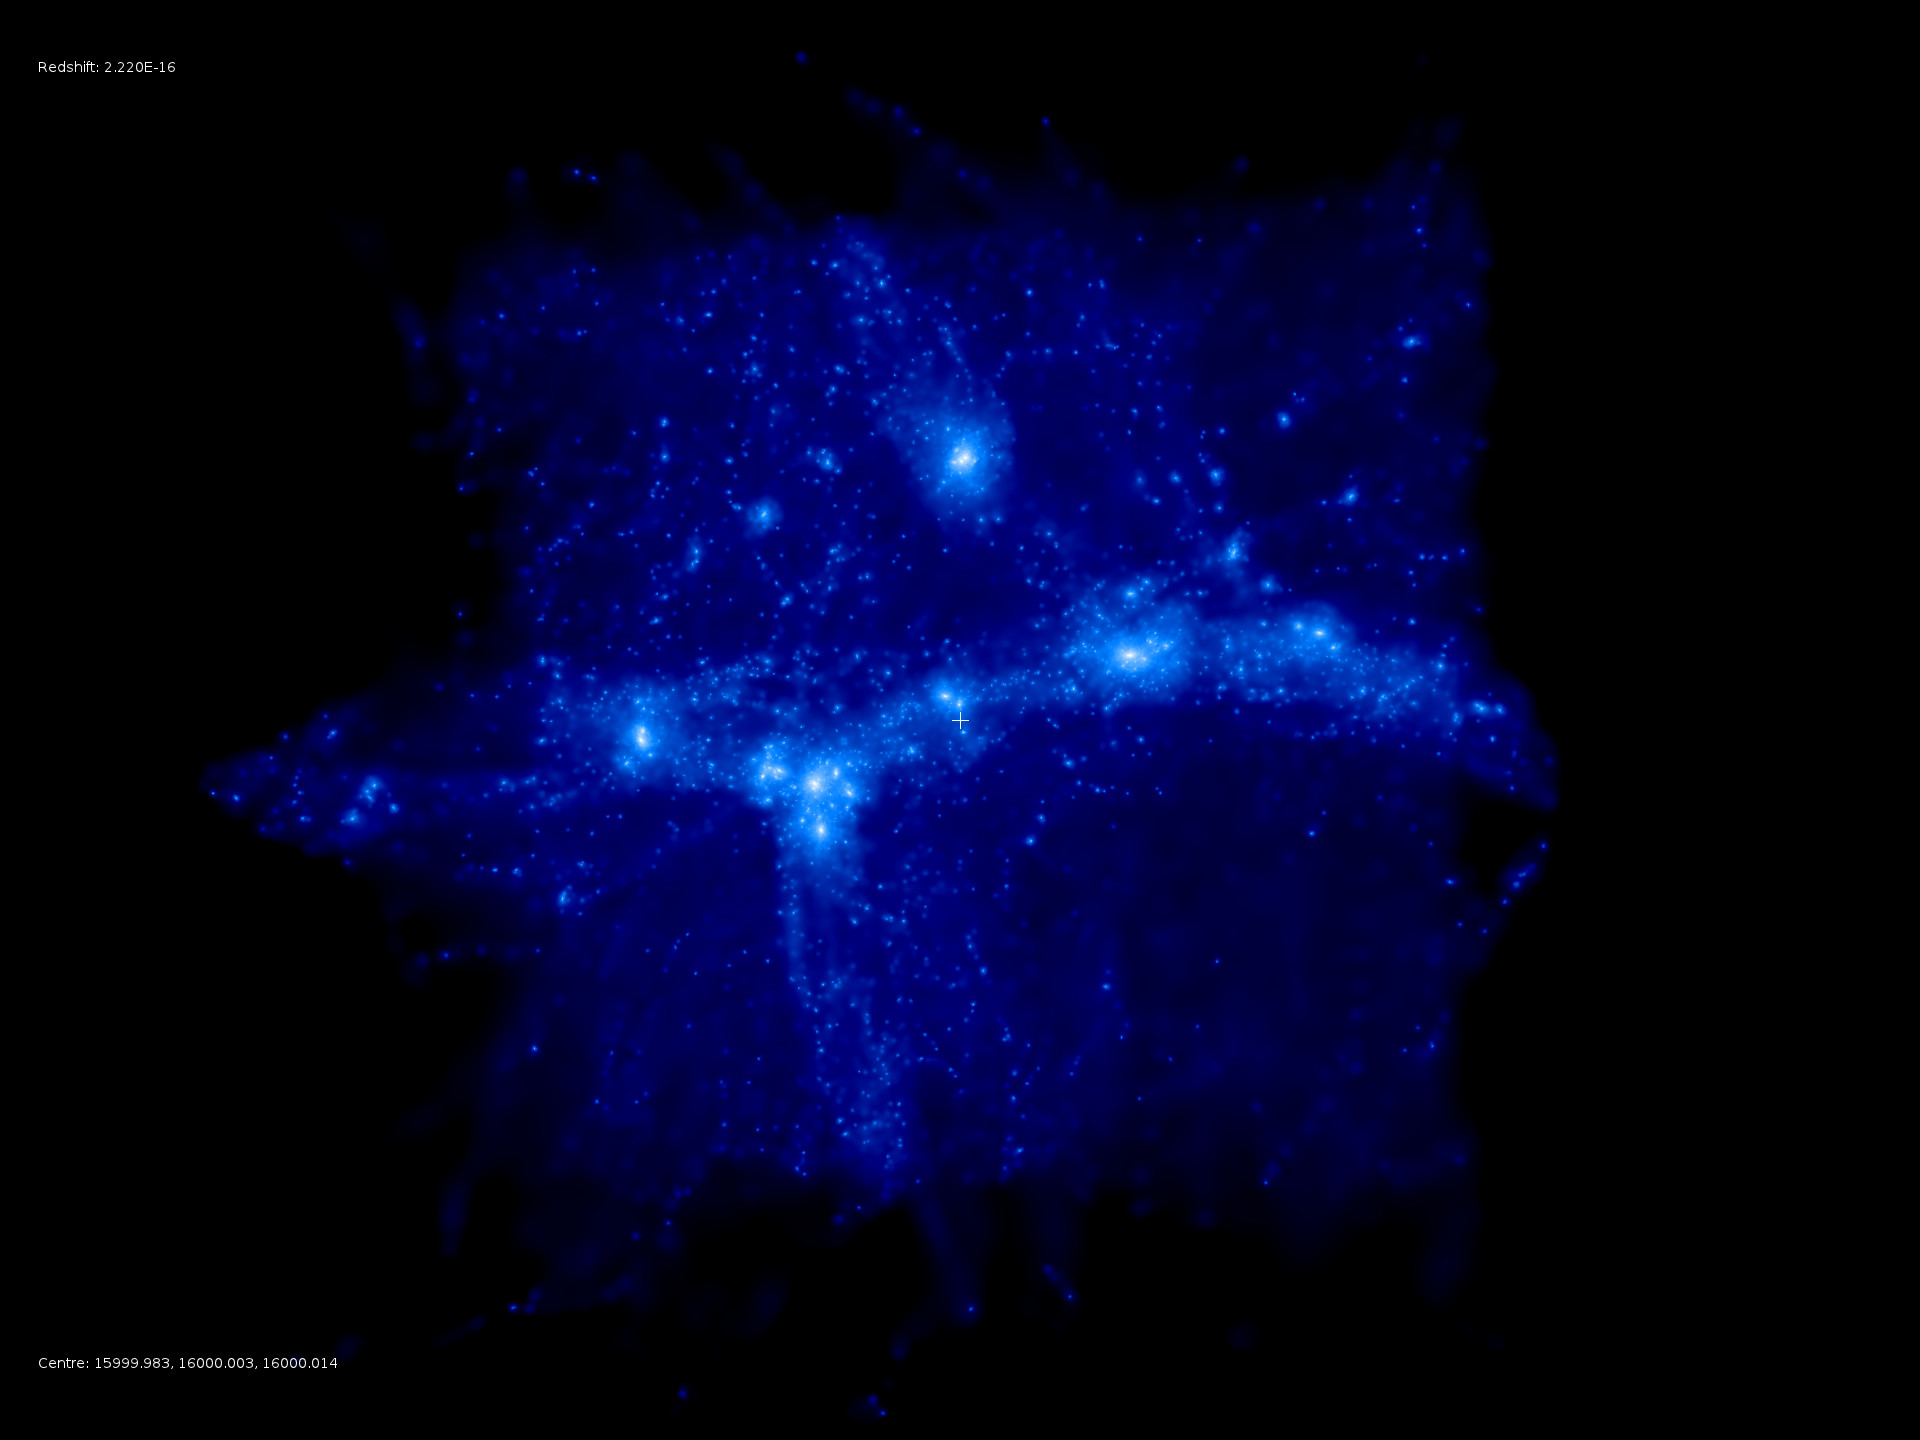
\includegraphics[scale=0.12]{r128/drdx_3/rotate_00185.jpg} 
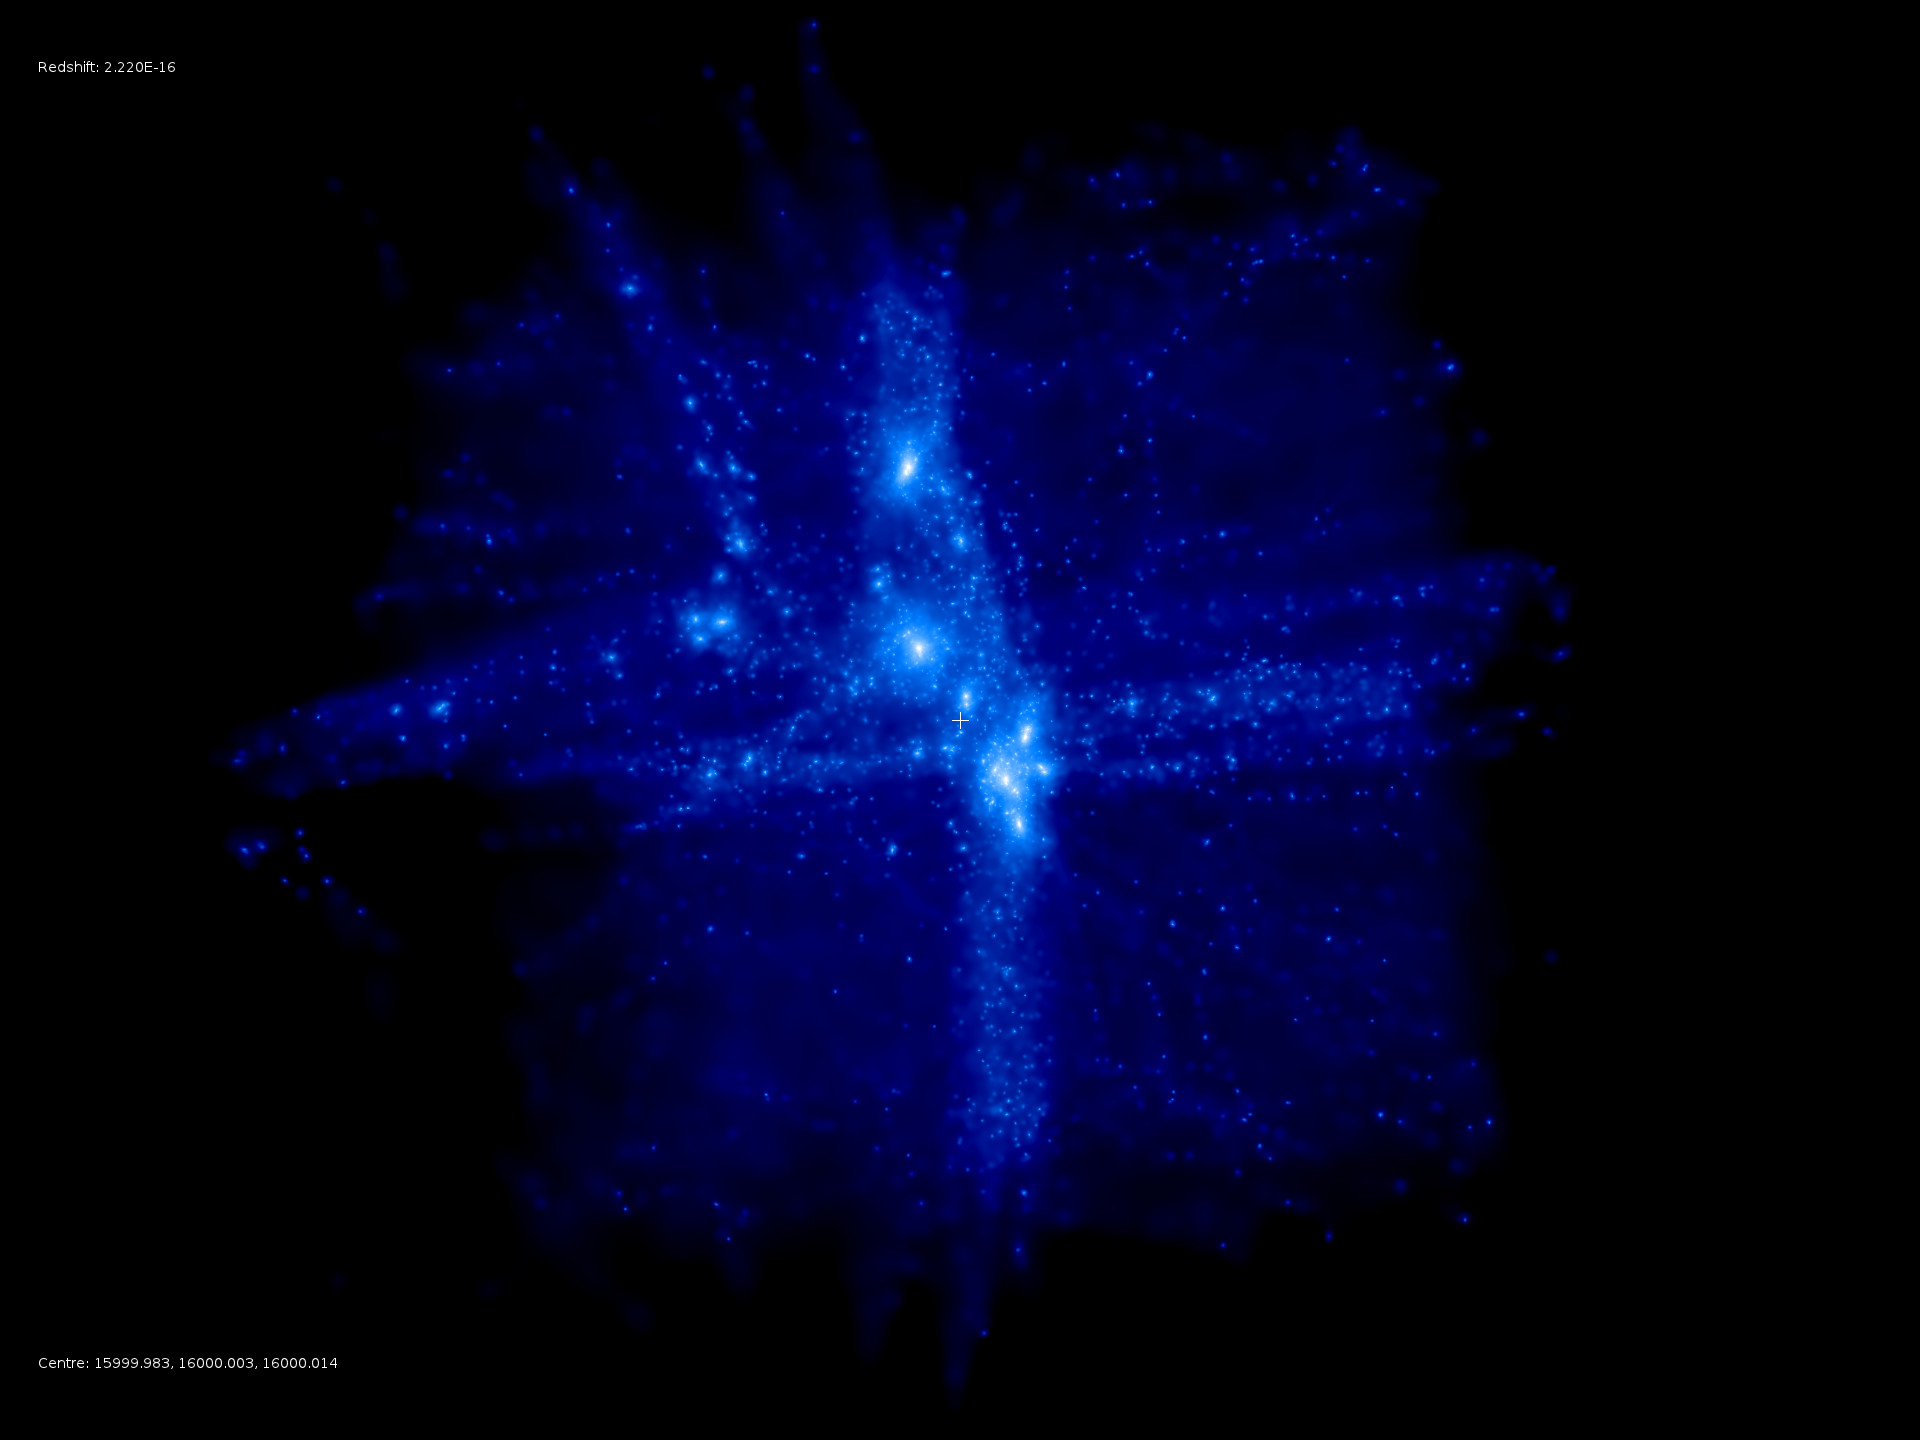
\includegraphics[scale=0.12]{r128/drdx_3/rotate_00136.jpg} 

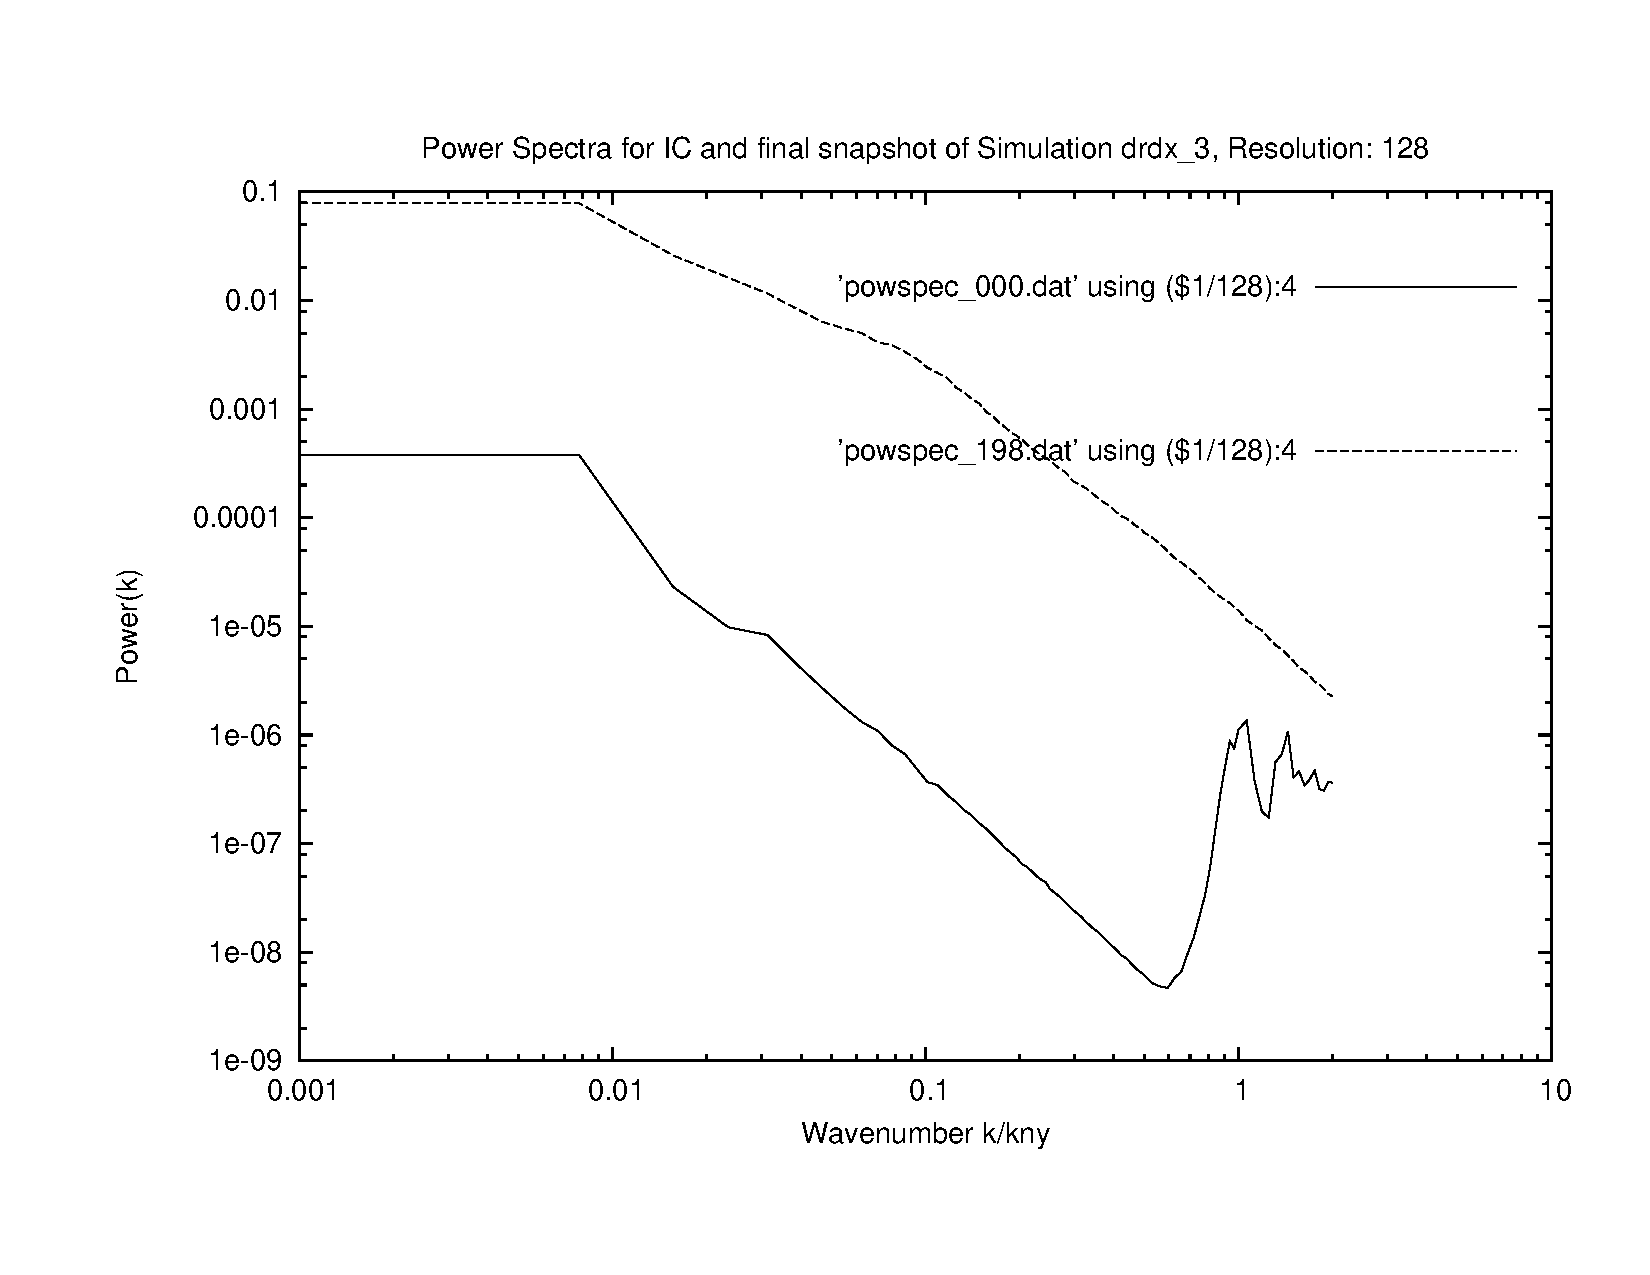
\includegraphics[scale=0.5]{r128/drdx_3/plot_powspec_drdx_3.pdf}


\textsc{rockstarred} $\surd$  \\
pfff $\rightarrow$ Error: too few halos at scale factor 0.926072 to calculate consistency metric.

\newpage
\subsection{drdx\_h100\_r128\_1}

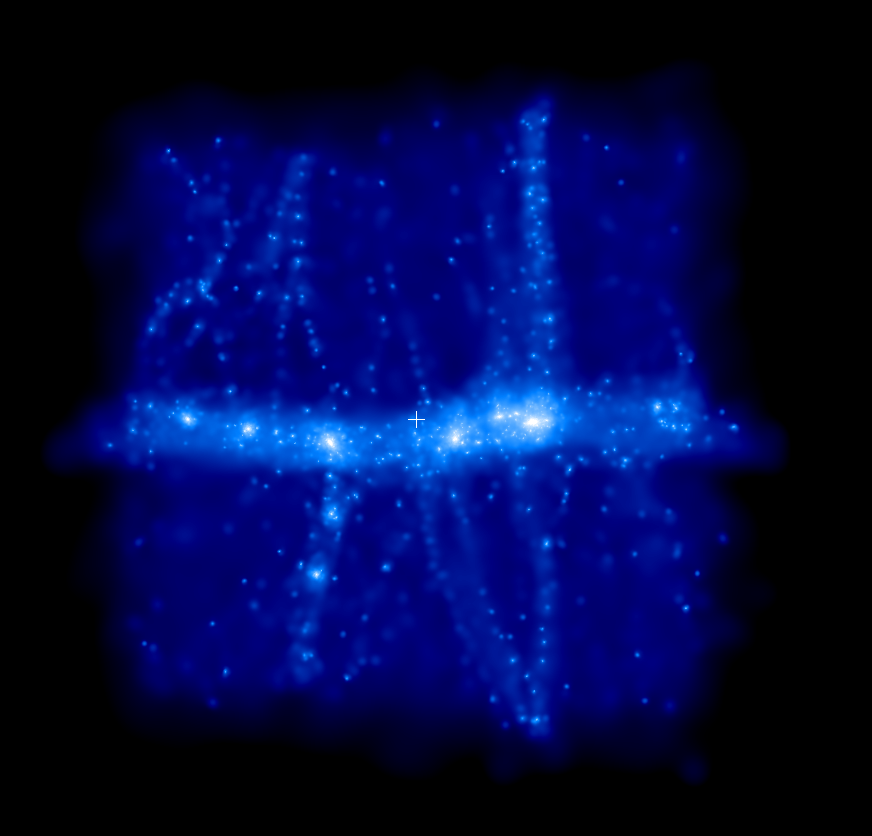
\includegraphics[scale=0.25]{r128/drdx_h100_r128_1/1.png} 
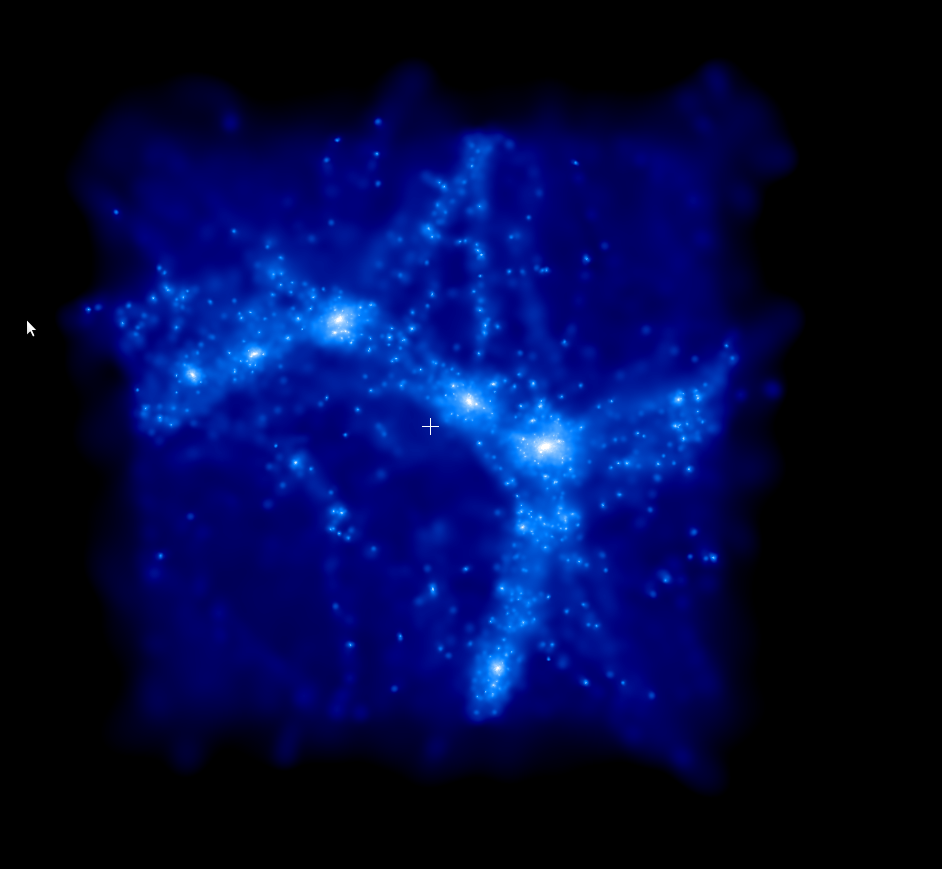
\includegraphics[scale=0.25]{r128/drdx_h100_r128_1/2.png} 

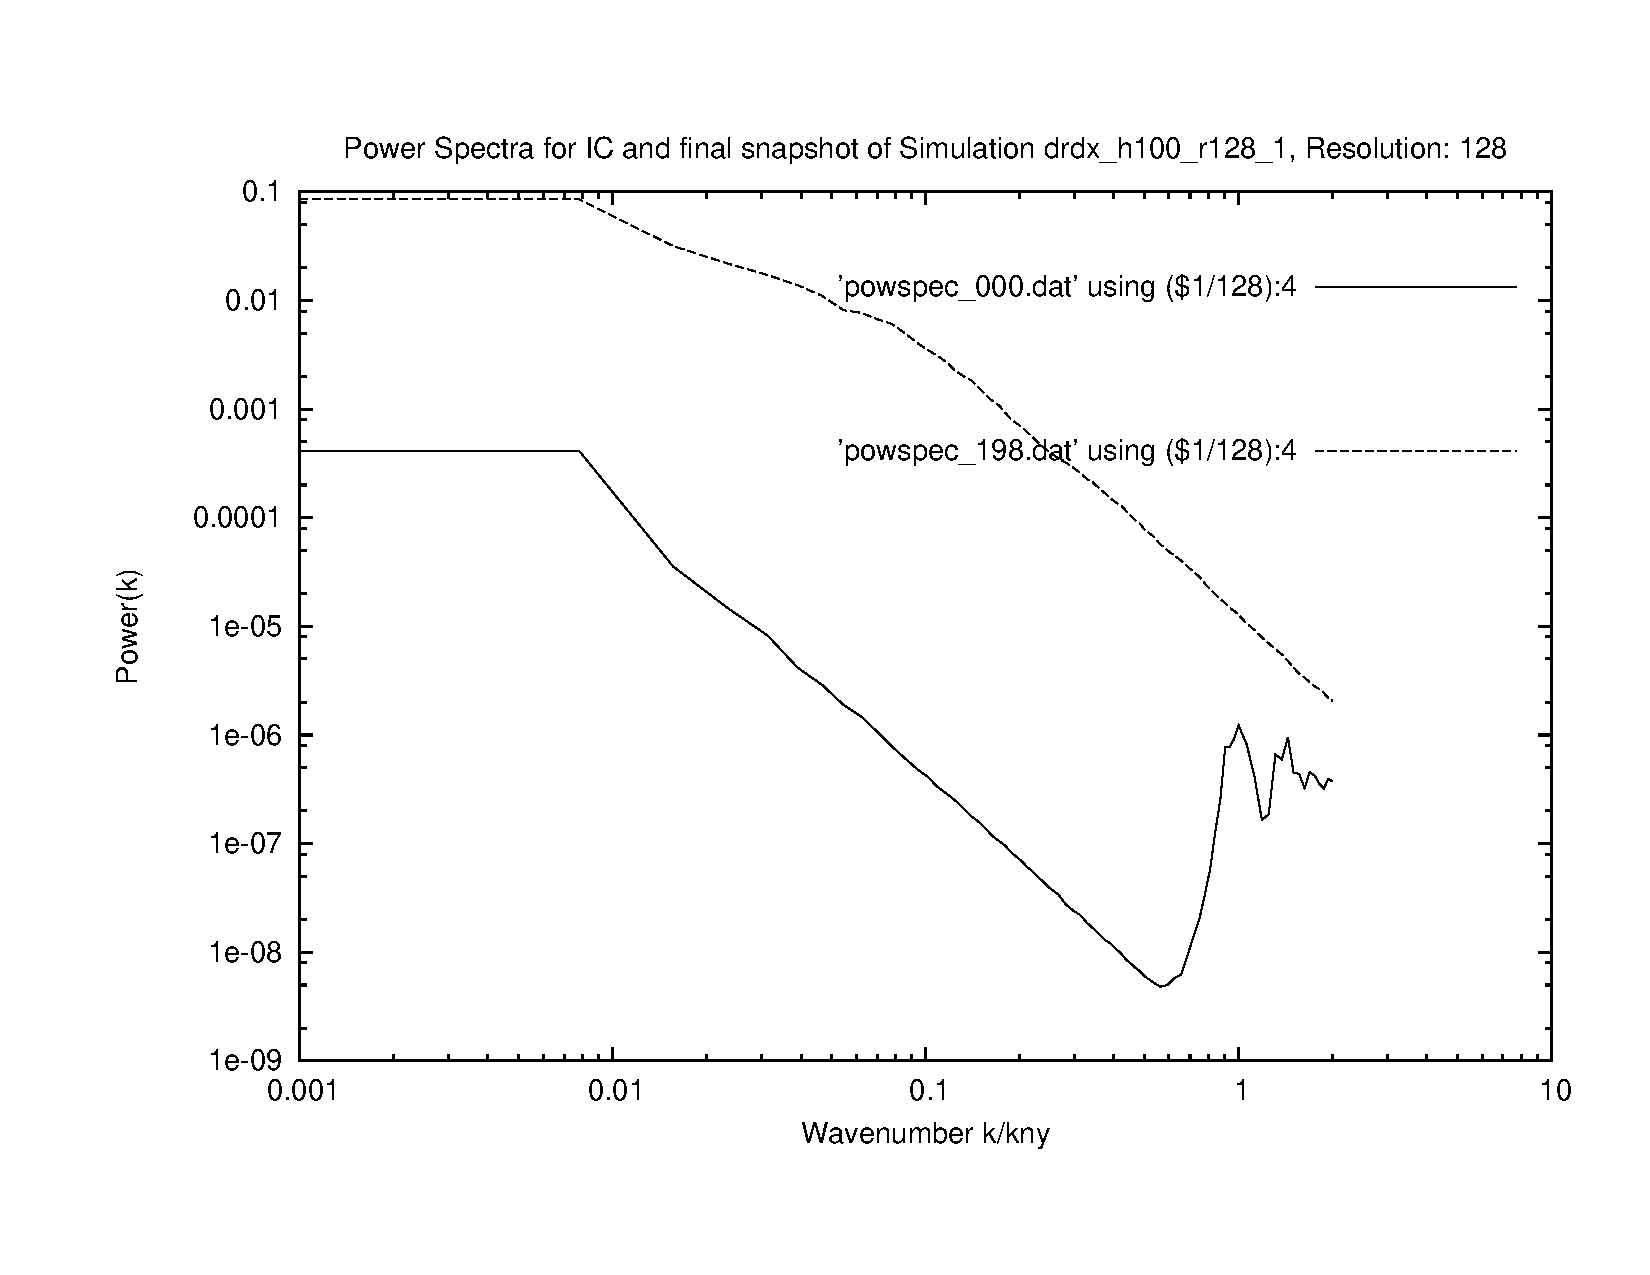
\includegraphics[scale=0.5]{r128/drdx_h100_r128_1/plot_powspec_drdx_h100_r128_1.pdf}


\textsc{rockstarred} $\surd$  \\
consistenttree: too few halos at scale factor 0.896 ... $\rightarrow$ wtf? 

\newpage
\subsection{drdx\_h100\_r128\_2}

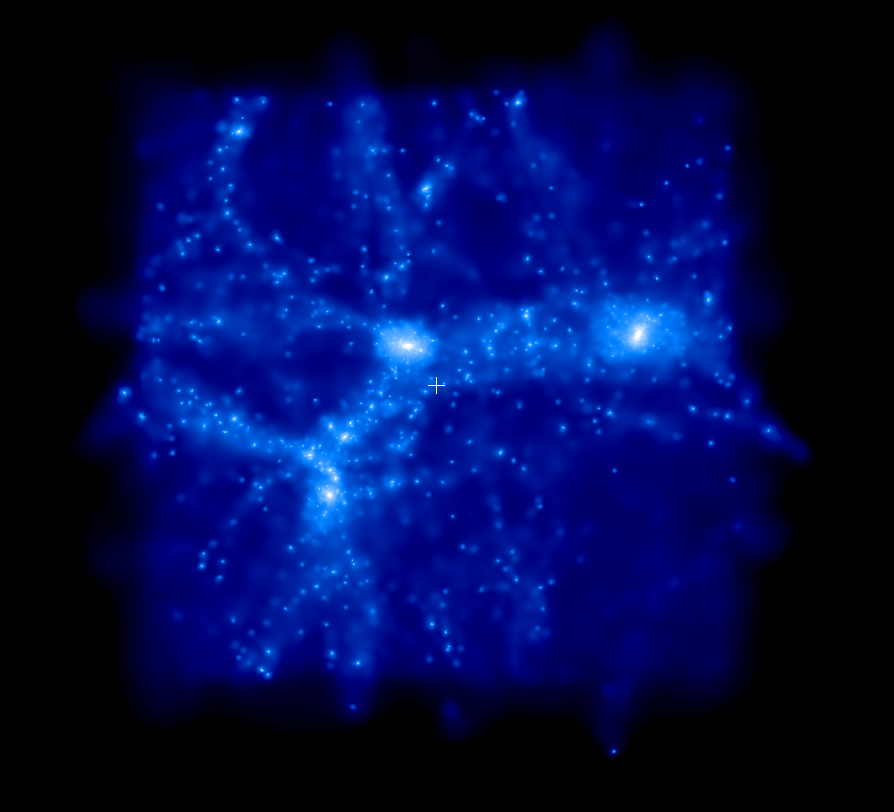
\includegraphics[scale=0.2]{r128/drdx_h100_r128_2/1.png} 
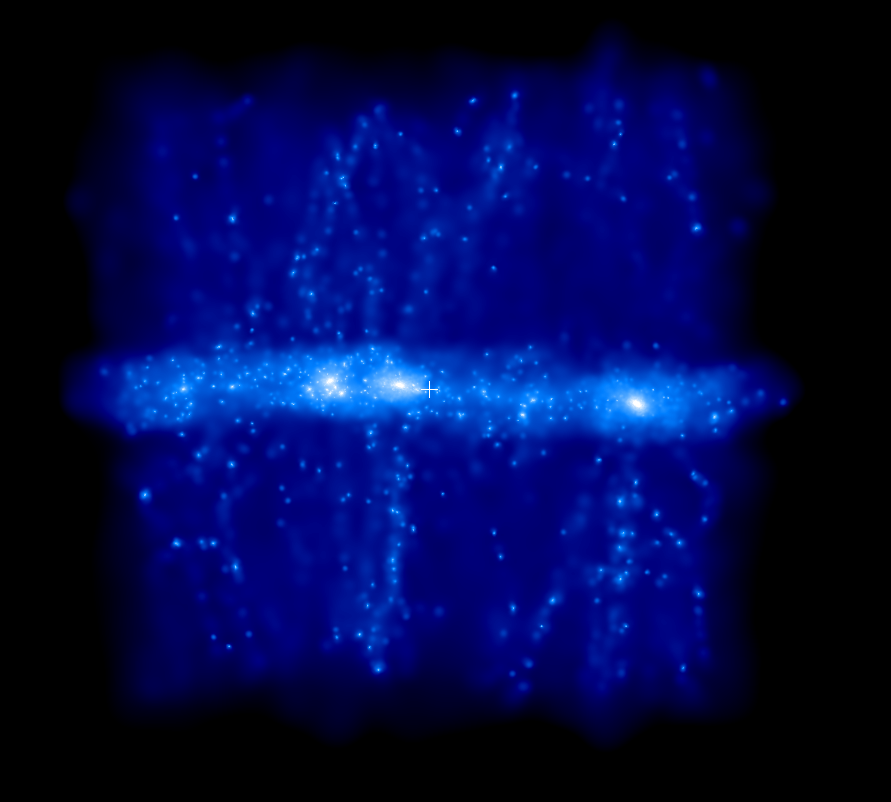
\includegraphics[scale=0.2]{r128/drdx_h100_r128_2/2.png} 

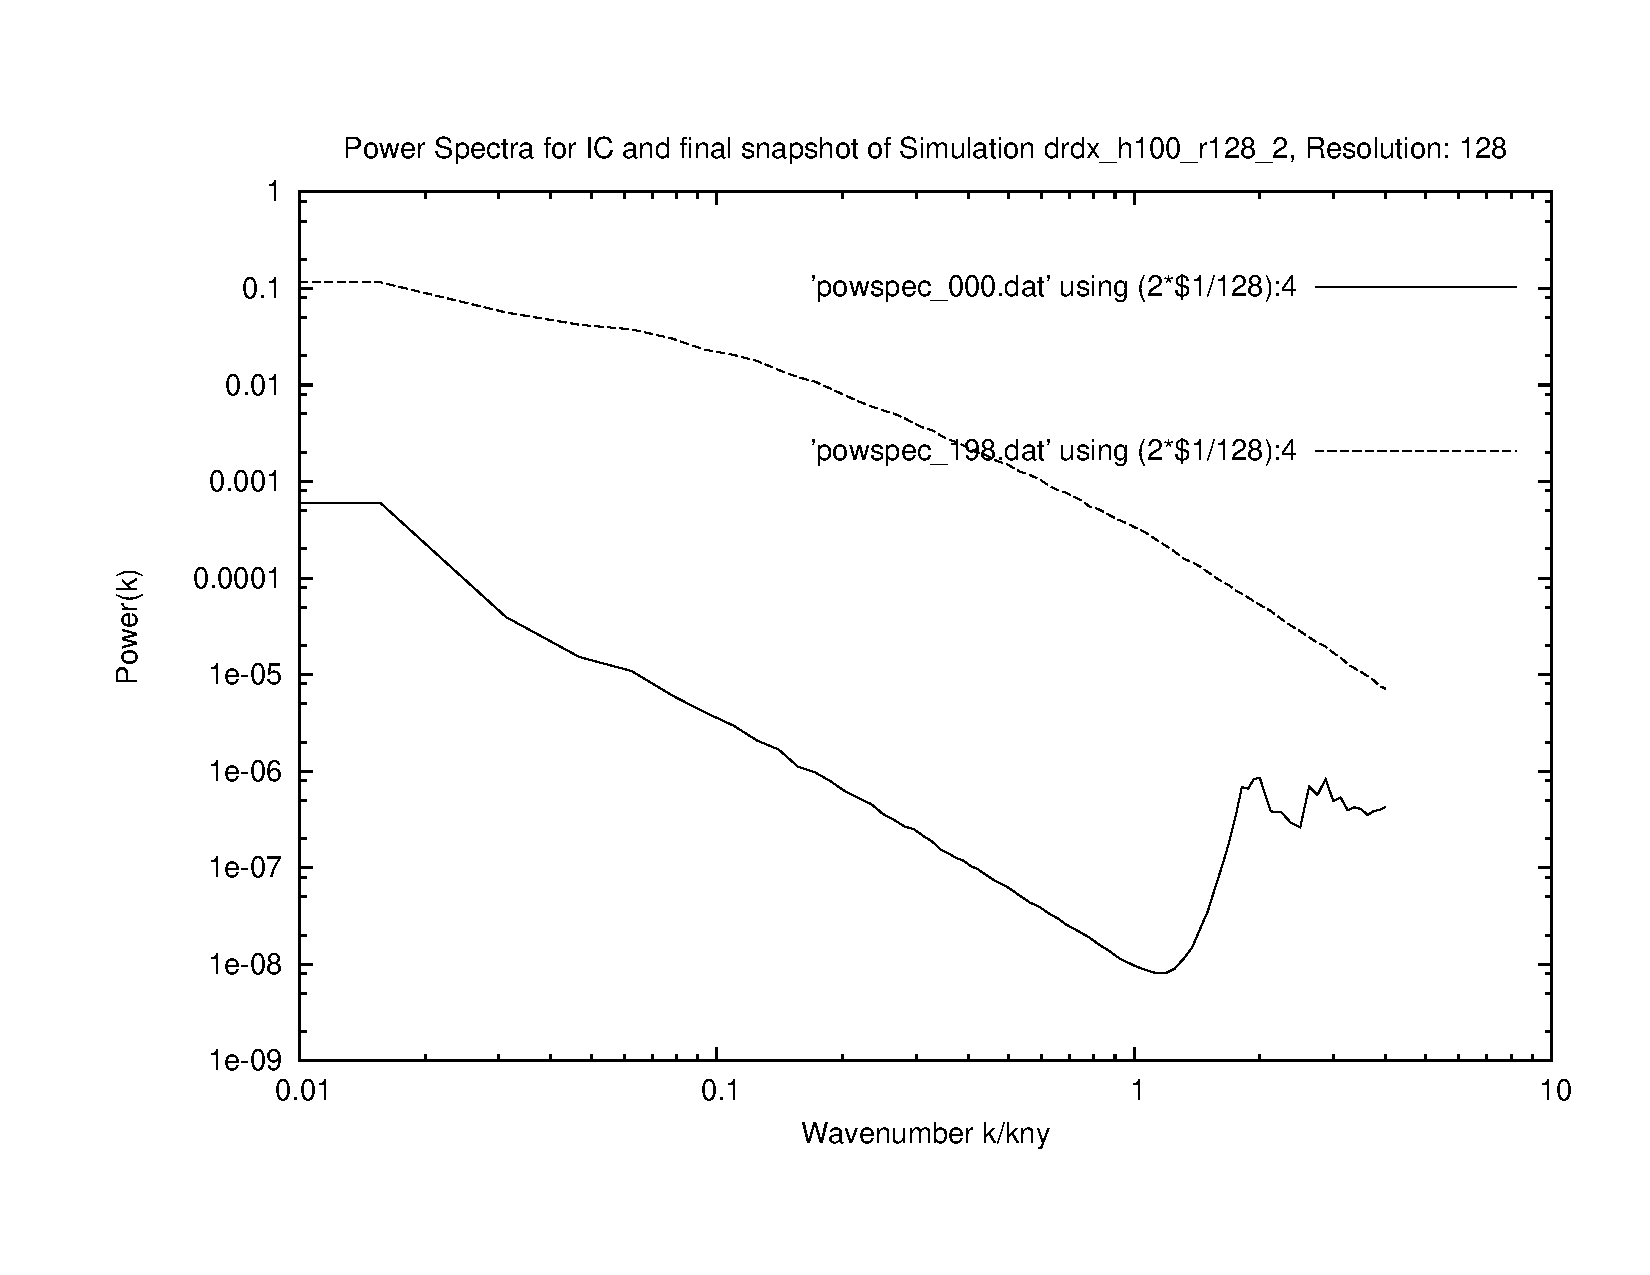
\includegraphics[scale=0.5]{r128/drdx_h100_r128_2/plot_powspec_drdx_h100_r128_2.pdf}




\newpage
\subsection{drkltest+3c+sl50\_1}
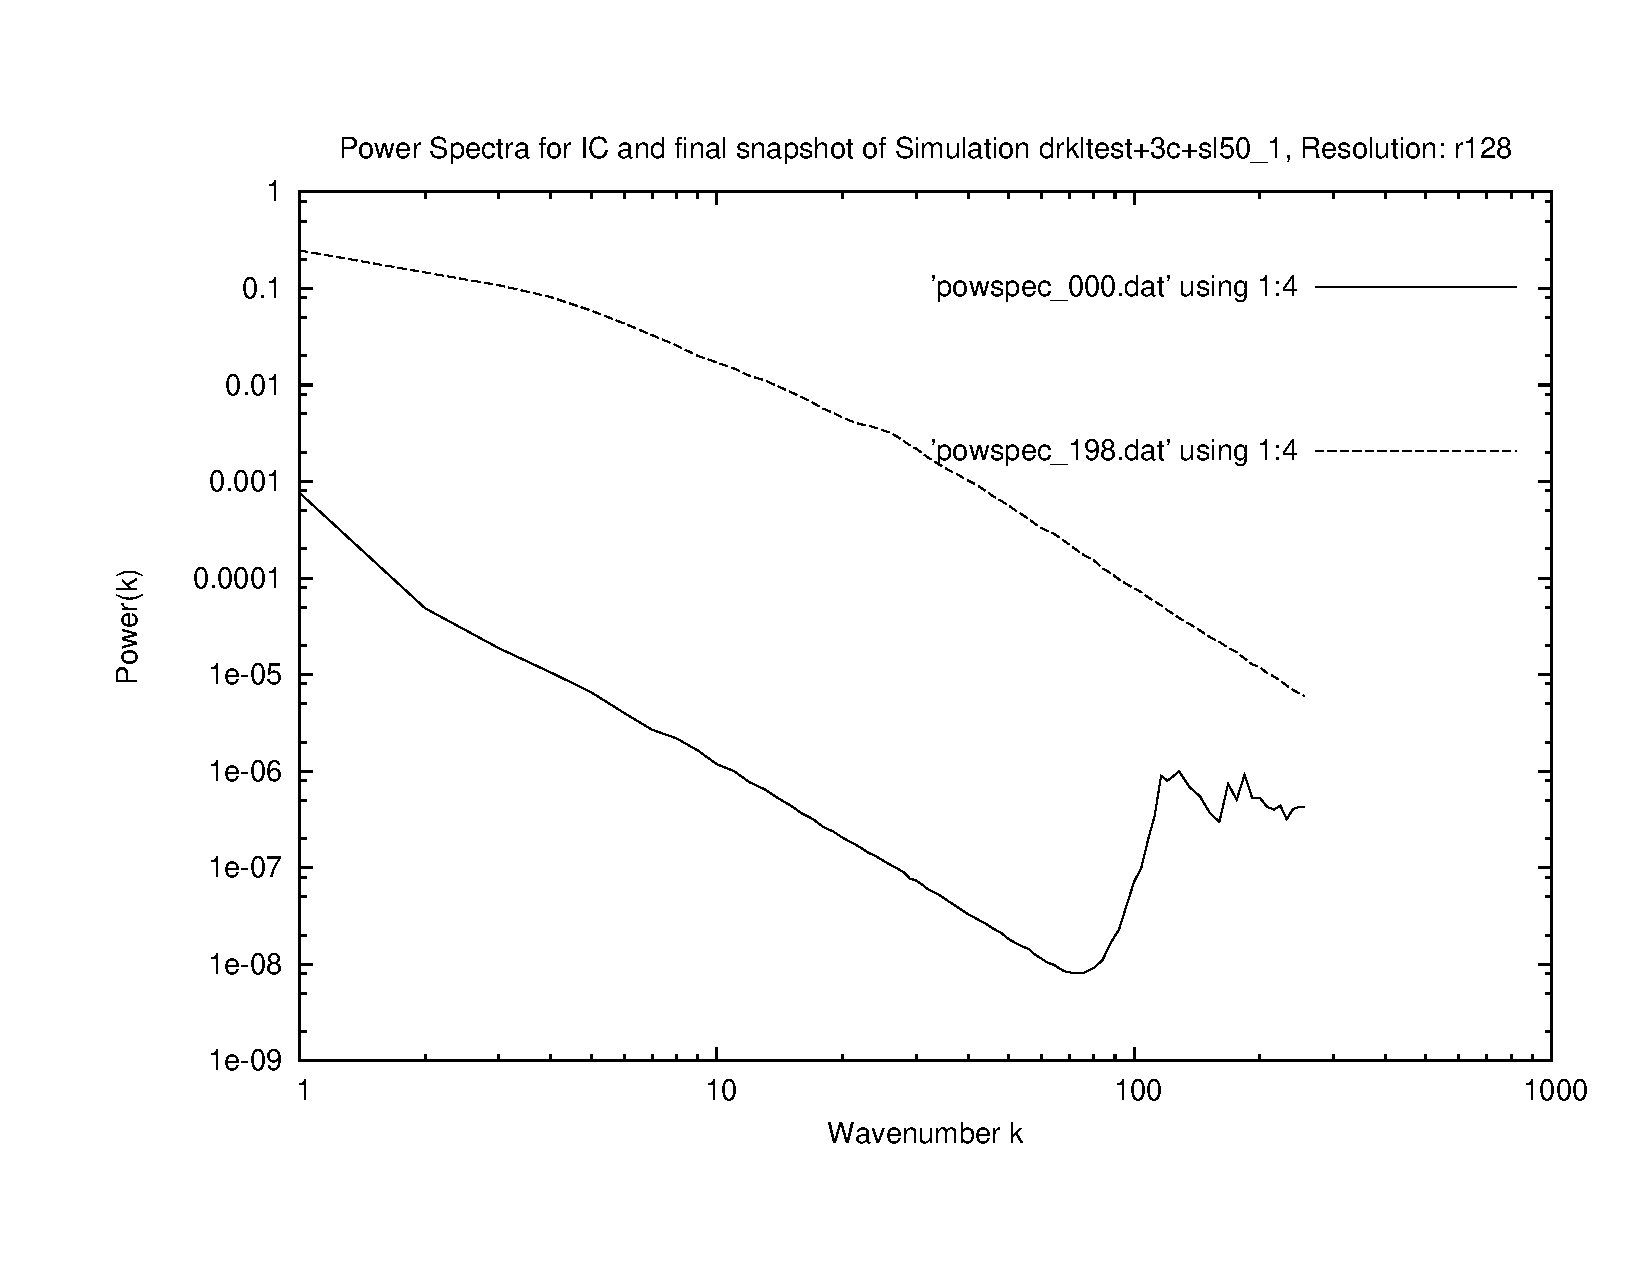
\includegraphics[scale=0.5]{r128/drkltest+3c+sl50_1/plot_powspec_drkltest+3c+sl50_1.pdf}


\begin{verbatim}
Error: too few halos at scale factor 0.890265 to calculate consistency metric.
Please remove this and all earlier timesteps from the scale file and rerun.
(DescScales.txt)
\end{verbatim}

\newpage

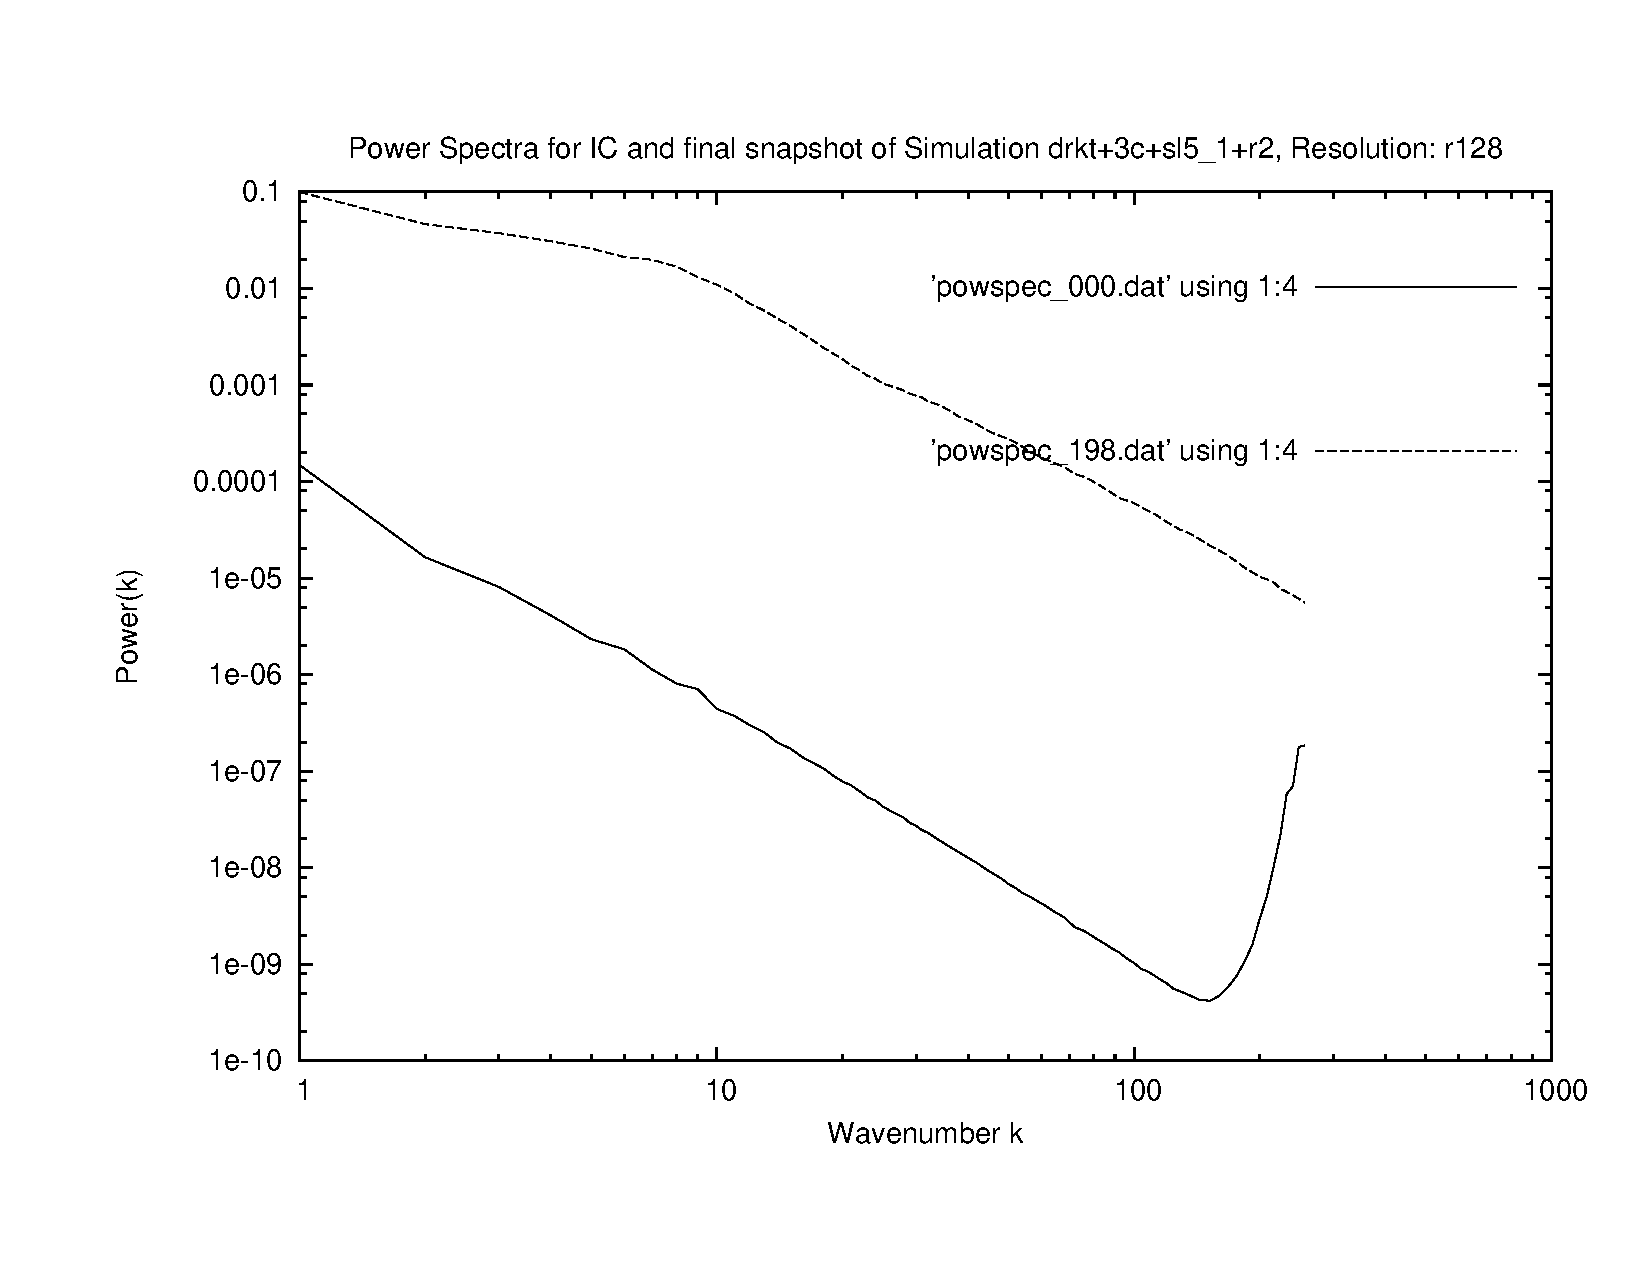
\includegraphics[scale=0.5]{r128/drkt+3c+sl5_1+r2/plot_powspec_drkt+3c+sl5_1+r2.pdf} \\
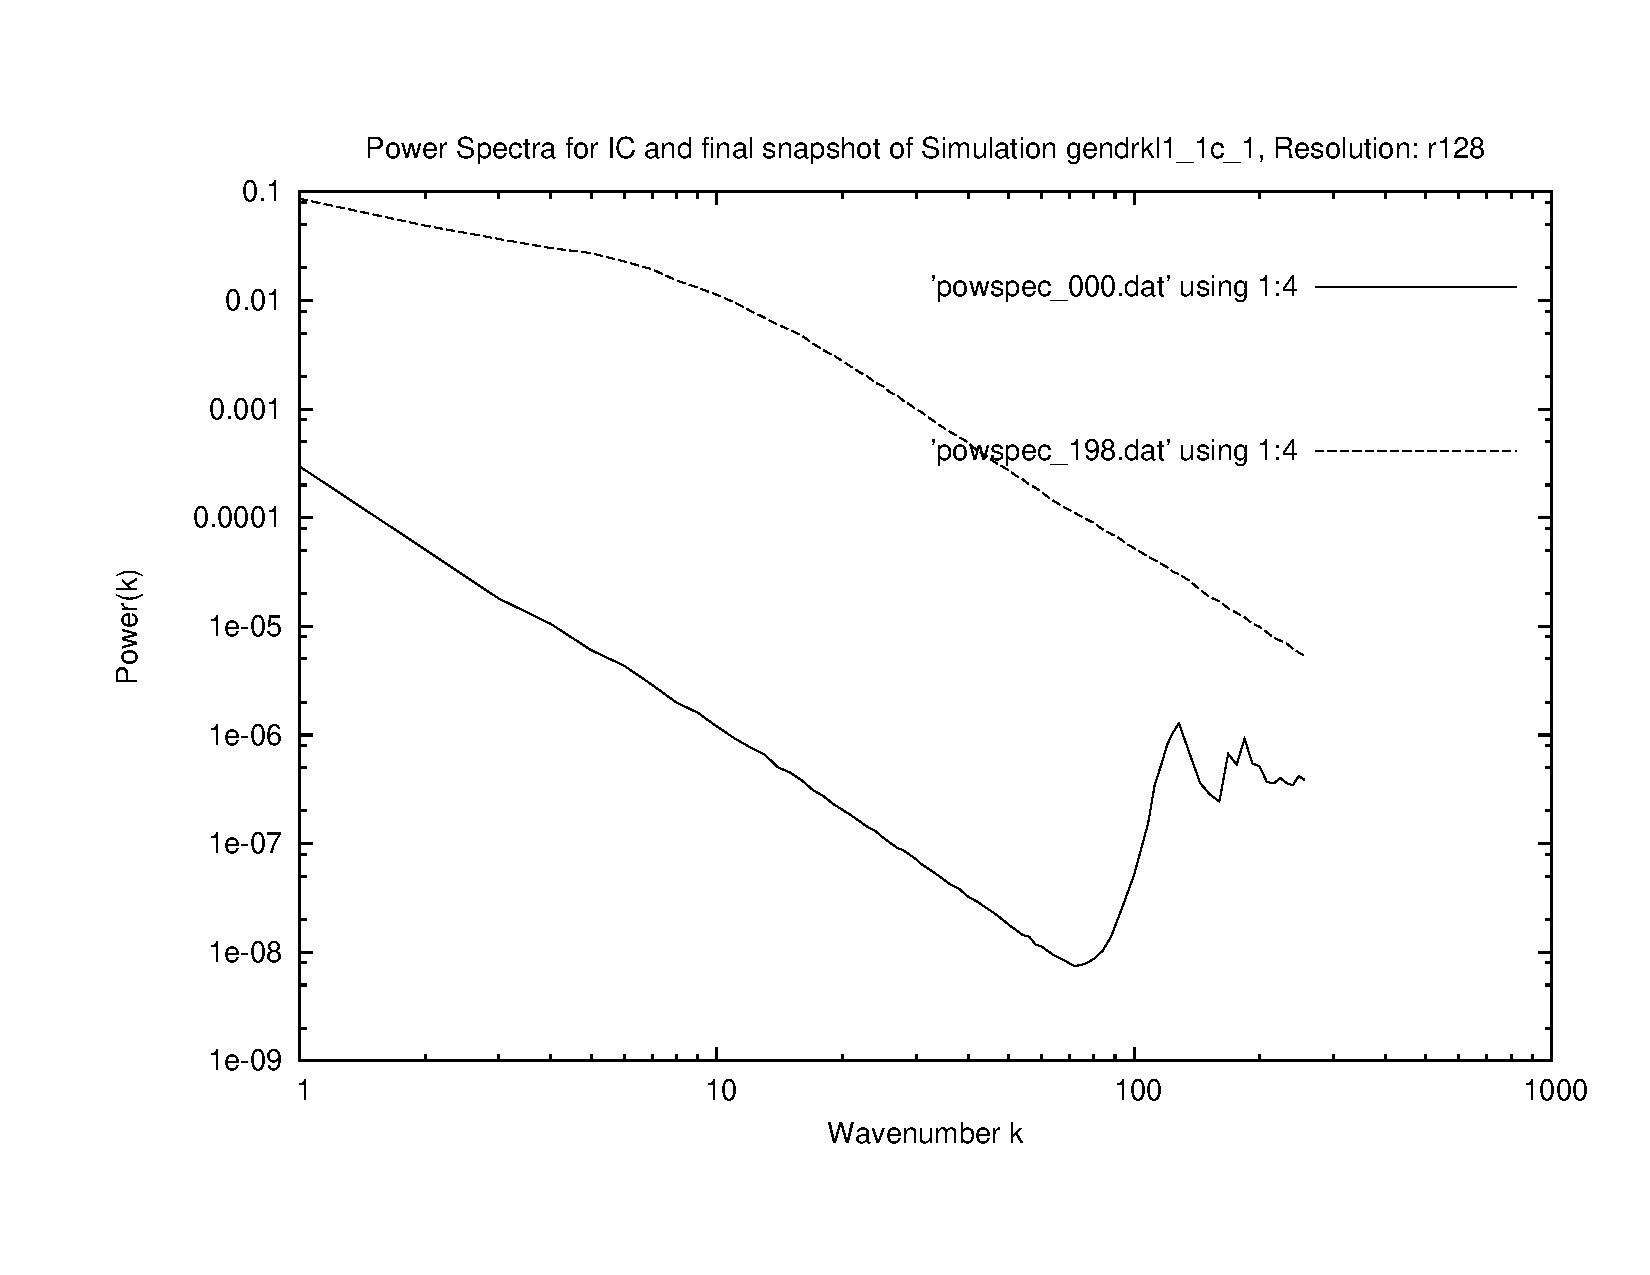
\includegraphics[scale=0.5]{r128/gendrkl1_1c_1/plot_powspec_gendrkl1_1c_1.pdf} \\
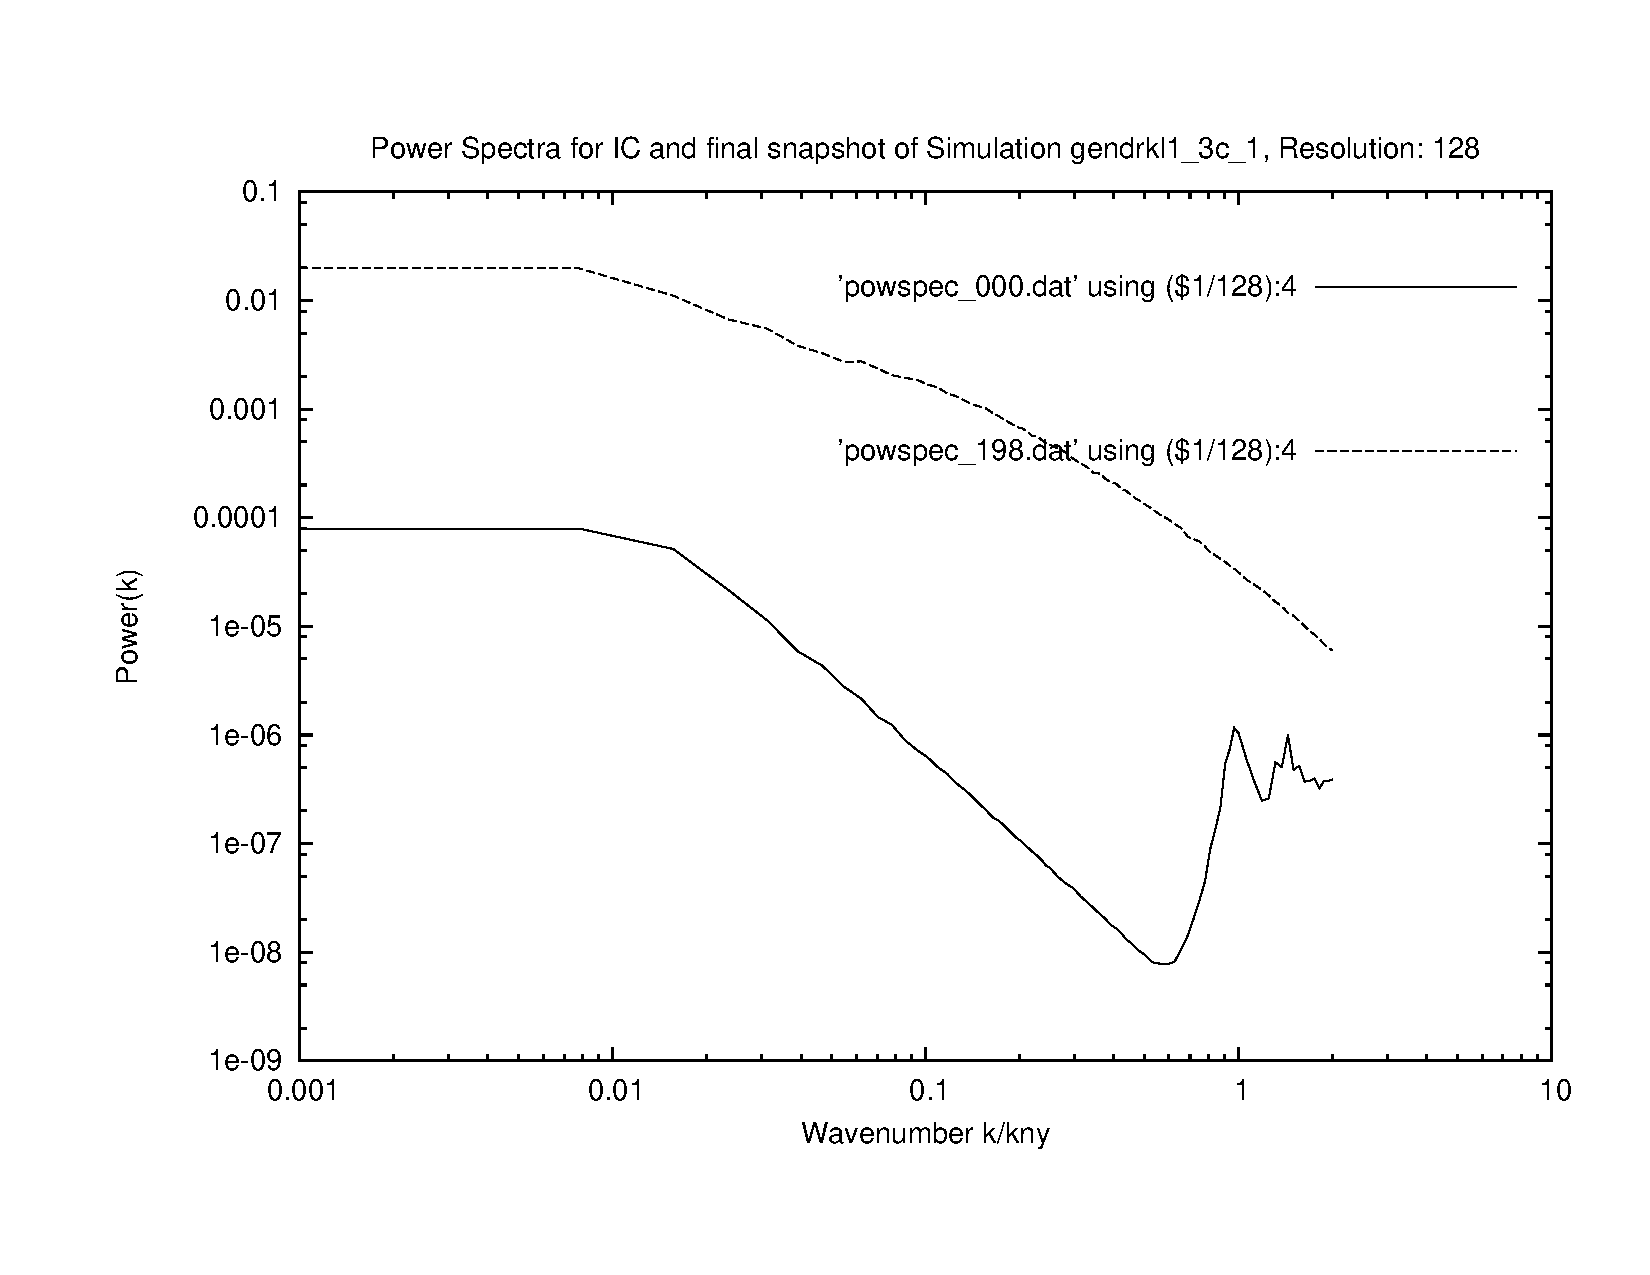
\includegraphics[scale=0.5]{r128/gendrkl1_3c_1/plot_powspec_gendrkl1_3c_1.pdf}